\documentclass{article}
\usepackage[utf8]{inputenc}
\usepackage{amsmath}
\usepackage{tcolorbox}
\usepackage{amssymb}
\usepackage{amsthm}
\usepackage{proof}
\theoremstyle{definition}


\usepackage[
top    = 2.50cm,
bottom = 2.50cm,
left   = 2.75cm,
right  = 2.75cm]{geometry}
\usepackage{fancyhdr}
\pagestyle{fancy}
\lhead{Advanced computation}
\rhead{EPFL/Alp Ozen}


\title{Advanced Computation}
\author{alp.ozen}
\date{\vspace{-5ex}}
\newtheorem{theorem}{Theorem}[section]
\newtheorem{example}{Example}
\newtheorem{definition}{Definition}
\newtheorem{question}{Question \textit{???}}
\begin{document}

\maketitle
\section{Propositional logic }
\subsection{Propositions}
A proposition is a declarative sentence that is either true or false. 
\begin{tcolorbox}
How much does it cost? \textbf{is not a proposition}
\\
I like red \textbf{is a proposition}
\end{tcolorbox}

To make life easier, we represent propositional statements through letters such as $p$. 
\\

The conditional statement $p\implies q$ appears very often. Thus, we have the \textit{converse,contrapositive and inverse} which are:
\\
\textbf{converse}: $q \implies p$
\\
\textbf{contrapositive}: $ \neg q \implies \neg p $
\\
\textbf{inverse}: $ \neg p \implies \neg q$
\\

We note that a conditional is logically equivalent to its contrapositive. 

\begin{tcolorbox}
\centering
\begin{array}{cccccc}
 p & q & p $\implies$ q & \neg q & \neg p & \neg q $\implies$ \neg p \\
 \hline
t & t & t & f & f & t\\
t & f & f & t & f & f\\
f & t & t & f & t & t\\
f & f & t & t & t & t
\end{array}
\end{tcolorbox}

\subsection{Precedence of logical operators}

\begin{figure}[h]
    \centering
    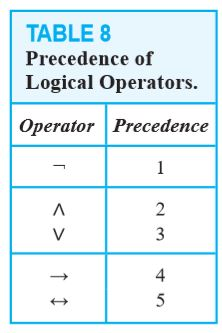
\includegraphics{figures/precedence}
\end{figure}

\subsection{Fuzzy logic}

In fuzzy logic, truth values are between 0 and 1. So if the statement "I like riding a bike" has a value of 0.8, it's negation has 1 minus this value, in this case -0.2. 

\subsection{Applications of logic}
\subsubsection{Logic gates}
Here are the basic logic circuits from which more complex circuits are made: 

\begin{figure}[h]
    \centering
    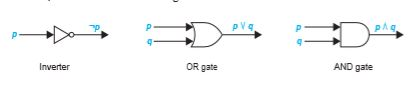
\includegraphics[scale= 1]{epflSemesterOne/advancedComputation/figures/logicgates.JPG}
    \caption{Logic gates}
    \label{fig:my_label}
\end{figure}

Note that the OR and AND gates accept only and only 2 inputs and output one. This input may be as compounded as possible but not exceed 'two chunks'. Thus, when given a complex logical output and reverse engineering, we identify the outer most outer operation, branch it into two or one(if it is simply a negation) and so on. 

\subsubsection{More on propositions}

\begin{tcolorbox}
\begin{itemize}
    \item \textbf{Tautology} is a compound proposition that is always true regardless of the truth value of its variables
    \item \textbf{Contradiction} is a compound proposition that is always false regardless of the truth value of its variables 
    \item \textbf{Contingency} compound statement that is neither tautology nor contradiction
    
    \begin{example}
    \\
    $p \land \neg p$ is a contradiction
    \\
    $p \lor \neg p$ is a tautology
    \end{example}
\end{itemize}
\end{tcolorbox}

Here are some examples of logical calculus:
\\
Show that $\neg(p \lor (\neg p \land q )) \equiveq \neg p \land \neg q$
\begin{align*}
    \neg(p\lor\neg p \land p \lor q)\\
    \neg(T \land p \lor q)\\
    \neg(p \lor q)\\
    \neg p \land \neg q
\end{align*}

\subsubsection{Satisfiability}

A compound proposition is \textbf{satisfiable} if a truth assignment can be made to its variables that make it true making it either a tautology or a contingency. It is \textbf{unsatisfiable} if the negation of the compound statement is a contradiction. 

\subsection{Logical calculus and useful equivalences}

\begin{definition}
If $A \iff B$ is a tautology, then A is logically equivalent to B. 
\end{definition}
\\

Here are some useful logical equivalences(omitting most obvious ones):

\begin{align*}
    p \implies q \equiv \neg p \lor q \equiv \neg(\neg q \lor p) \equiv \not(q \implies p) \equiv \neg q \implies \neg p \\
    p \lor ( q \land r) \equiv (p \lor q) \land (p \lor r) \\
    \land \ \text{distributes over} \lor \text{and vice versa}\\
    p \lor \neg p \equiv T\\
    p \land \neg p \equiv F\\
    P \land T \equiv p\\
    p \lor F \equiv p
    \text{both $\land$ and $\lor$ are associative}
\end{align*}

For more see this figure:

\begin{figure}[h]
    \centering
    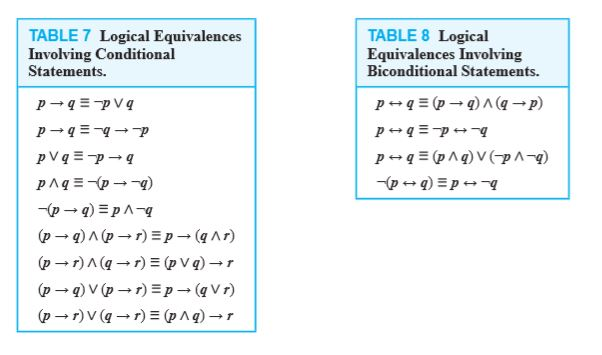
\includegraphics[scale = 0.7]{epflSemesterOne/advancedComputation/figures/logic.JPG}
    \caption{Logic, yey!}
    \label{fig:my_label}
\end{figure}

\begin{definition}
A \textbf{rule of inference} is based on the tautology $p \land (p \implies q) \implies q$. That is, whenever we are given that both $p$ and $p \implies q$ is true, we infer that q must be true. That is :
\\

\infer{q}{p & (p \implies q)}
\end{definition}


\begin{question}
Given propositional variables and truth values of the single variables for which the compound proposition takes a value, is there a way of deducing a compound proposition? 
\end{question}






\end{document}